\documentclass{jsarticle}
\usepackage{amsmath}
\usepackage{url}
\usepackage{graphicx}
\usepackage{here}
\usepackage{listings}
\lstset{
    basicstyle={\ttfamily\small}, %書体の指定
    frame=tRBl, %フレームの指定
    framesep=10pt, %フレームと中身(コード)の間隔
    breaklines=true, %行が長くなった場合の改行
    linewidth=12cm, %フレームの横幅
    lineskip=-0.5ex, %行間の調整
    tabsize=2 %Tabを何文字幅にするかの指定
}

\begin{document}

\begin{titlepage}
    \begin{center}
        \vspace*{12pt}
        {\LARGE 計算機科学実験及び演習2(CADツール上での論理設計)}
        \vspace{12pt}\\
        {第3回}
        \vspace{60pt}\\
        {締め切り : 1月28日}
        \vspace{12pt}\\
        {提出日 : 1月26日}
    \end{center}

    \vspace{400pt}

    \begin{flushright}
       {\large 学籍番号: 1029300562\\
        氏名: 新山公太(にいやまこうた)}
    \end{flushright}

\end{titlepage}
\section{ALUの設計}
今回の課題は加減算及び基本的な論理演算を備えたALUを作ることであった。また、発展課題として比較、移動演算を備えることが要求された。今回はこれらすべての機能を備えたALUを作成したので、その仕様を満たしているか、また性能はどの程度であるかについてをレポートにまとめる。
なお、今回作ったALUは全加算器の繰り上げを順次次の加算器へと受け渡していく方式(桁上げ伝播方式)をとった。高速化するためには、桁上げ先見器を用いることが考えられるがこれは回路規模とのトレードオフとなる。
先見器を用いた構成は実際に設計をするところまではできなかったので、実際にシミュレーションした値で性能を比較することはできないので、文献をもとにどのくらいの性能差があるかを論述するにとどめる。
この際に参考にした文献については、巻末にまとめて示す。
\subsection{設計したALUの仕様}
配布されたプリントに記されている仕様の再掲となる部分も多いが、すべての入出力について説明していきたいと思う。
まずdataA,dataBはそれぞれ16ビットの入力であり、このデータをもとに演算が行われる。次にopcodeでは操作コードが指定され、配布資料にある通りに演算が指定される。なお、opcodeは4ビットの入力信号であるが、与えられた操作コードは7個であり、対応してない入力が存在する。そのようなものについては動作を保証していない。
対応してない入力に関してはエラーを返す仕様にすることもできたが、回路規模が多くなる恐れがあったので、今回はその機能を採用することはしなかった。

\subsection{シミュレーション結果}
\subsection{加算}
図1を見ればわかるようにちゃんと2進数の足し算が実現されている。condについてもすべてしっかりと判定できている。
また、線が赤色の所は冗談からの桁上げが伝播していないために計算が終わっていないところがあることを示している。
\begin{figure}
    \caption{加算}
  \includegraphics[scale=0.8]{ALU_add.ps}
\end{figure}
\subsection{減算}
減算はdataBの補数を取って加算を行っている。図を見れば正しい出力が得られていることがわかる。
なお、condのうち、桁上げを表すフラグが立っているが、上述の通り補数を取って加算をしているためである。
\begin{figure}
    \caption{減算}
  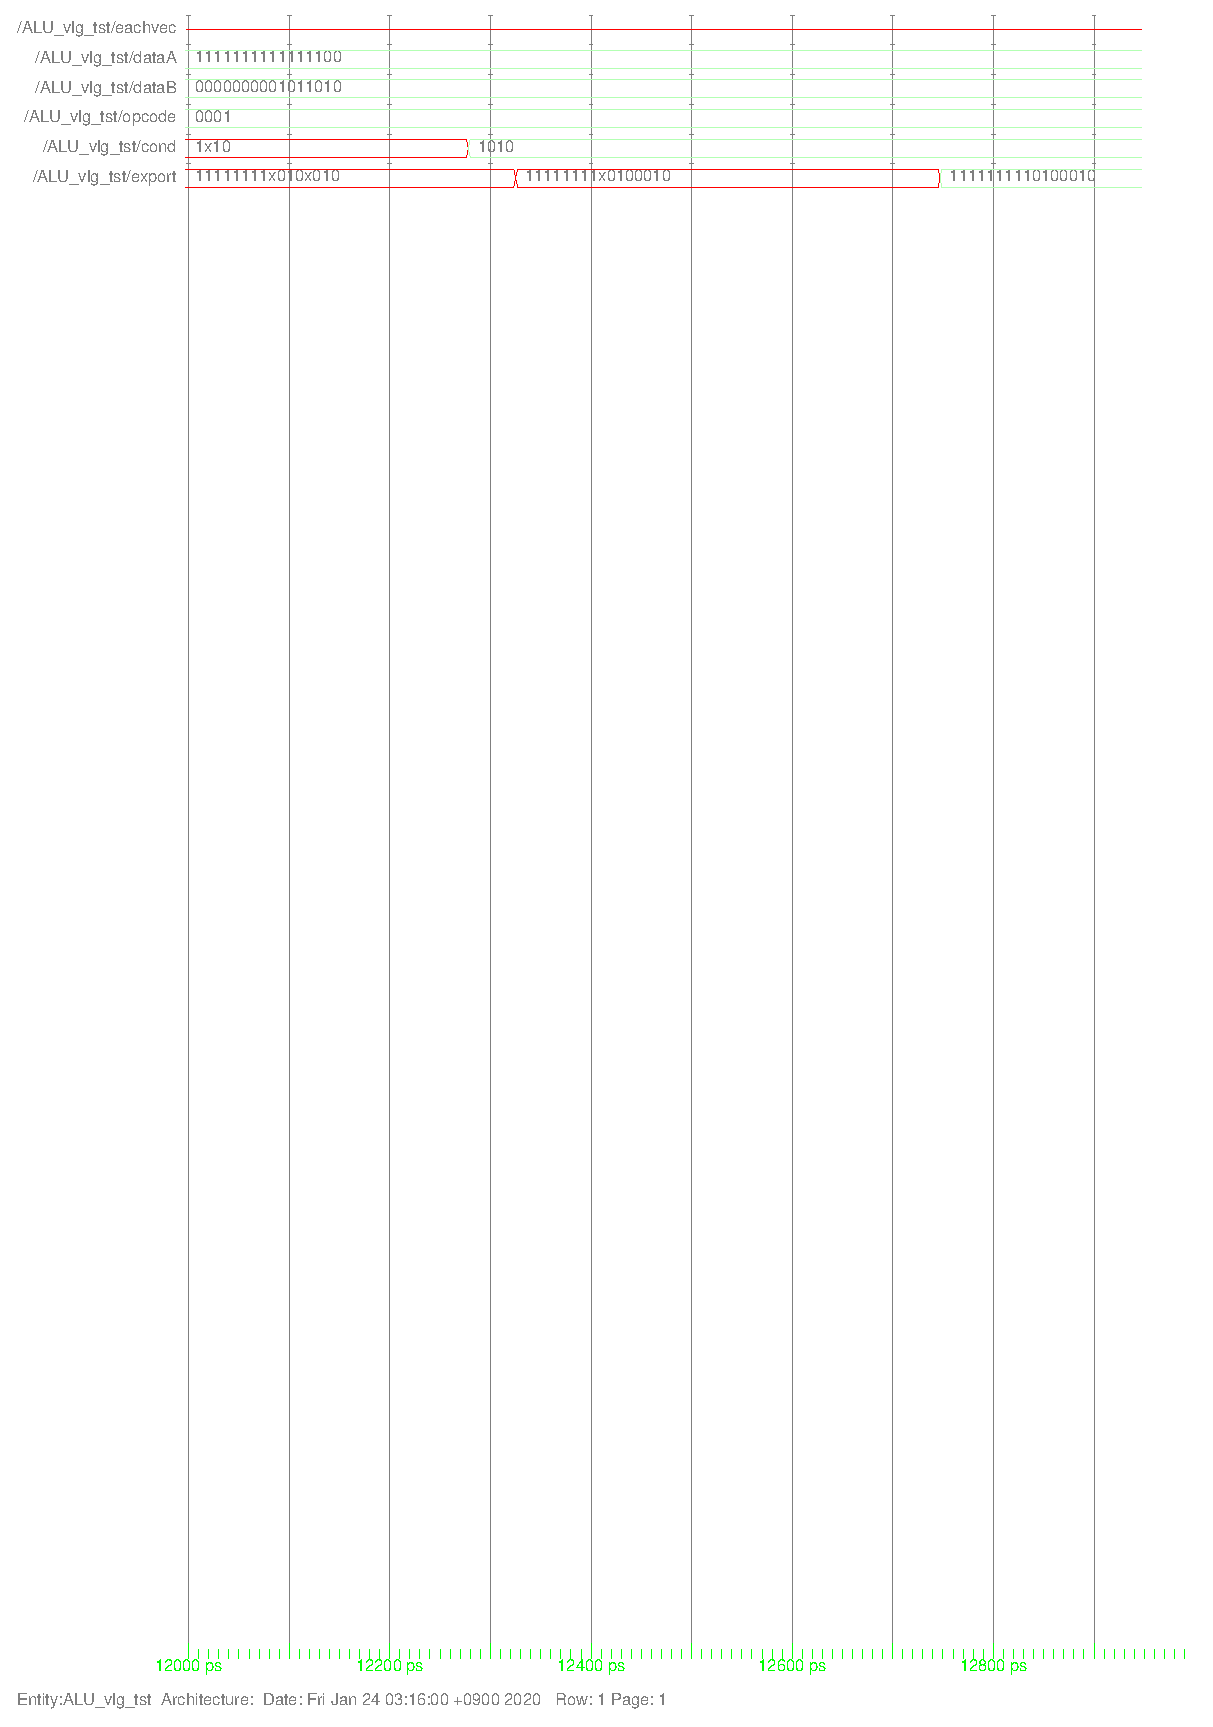
\includegraphics[scale=0.8]{ALU_subst.ps}
\end{figure}
\subsection{論理積}
出力に関しては図を見れば正しい答えが得られていることがわかる。気になるのは、オーバーフローのフラグがたっていることであるが、このALUの設計では操作コードによらず任意の演算を実行しておいて、後で操作コードによって採用する出力をマルチプレクサによって選択しているが、オーバーフローの判定は算術演算の結果を流用して行っており、論理演算が選択されたときについてはオーバーフローすることがないのでドントケアにしていたためである。
マルチプレクサを使って算術演算が選ばれたときと論理演算が選ばれたときで分岐させてもよいと思ったが、仕様を確認した結果ドントケアのままでも問題ないと判断した。
今回は回路規模がそんなに大きくないので問題にはならないが、意図してない入力による出力はドントケアとすることで回路規模を小さくすることができる。
\begin{figure}
    \caption{論理積}
  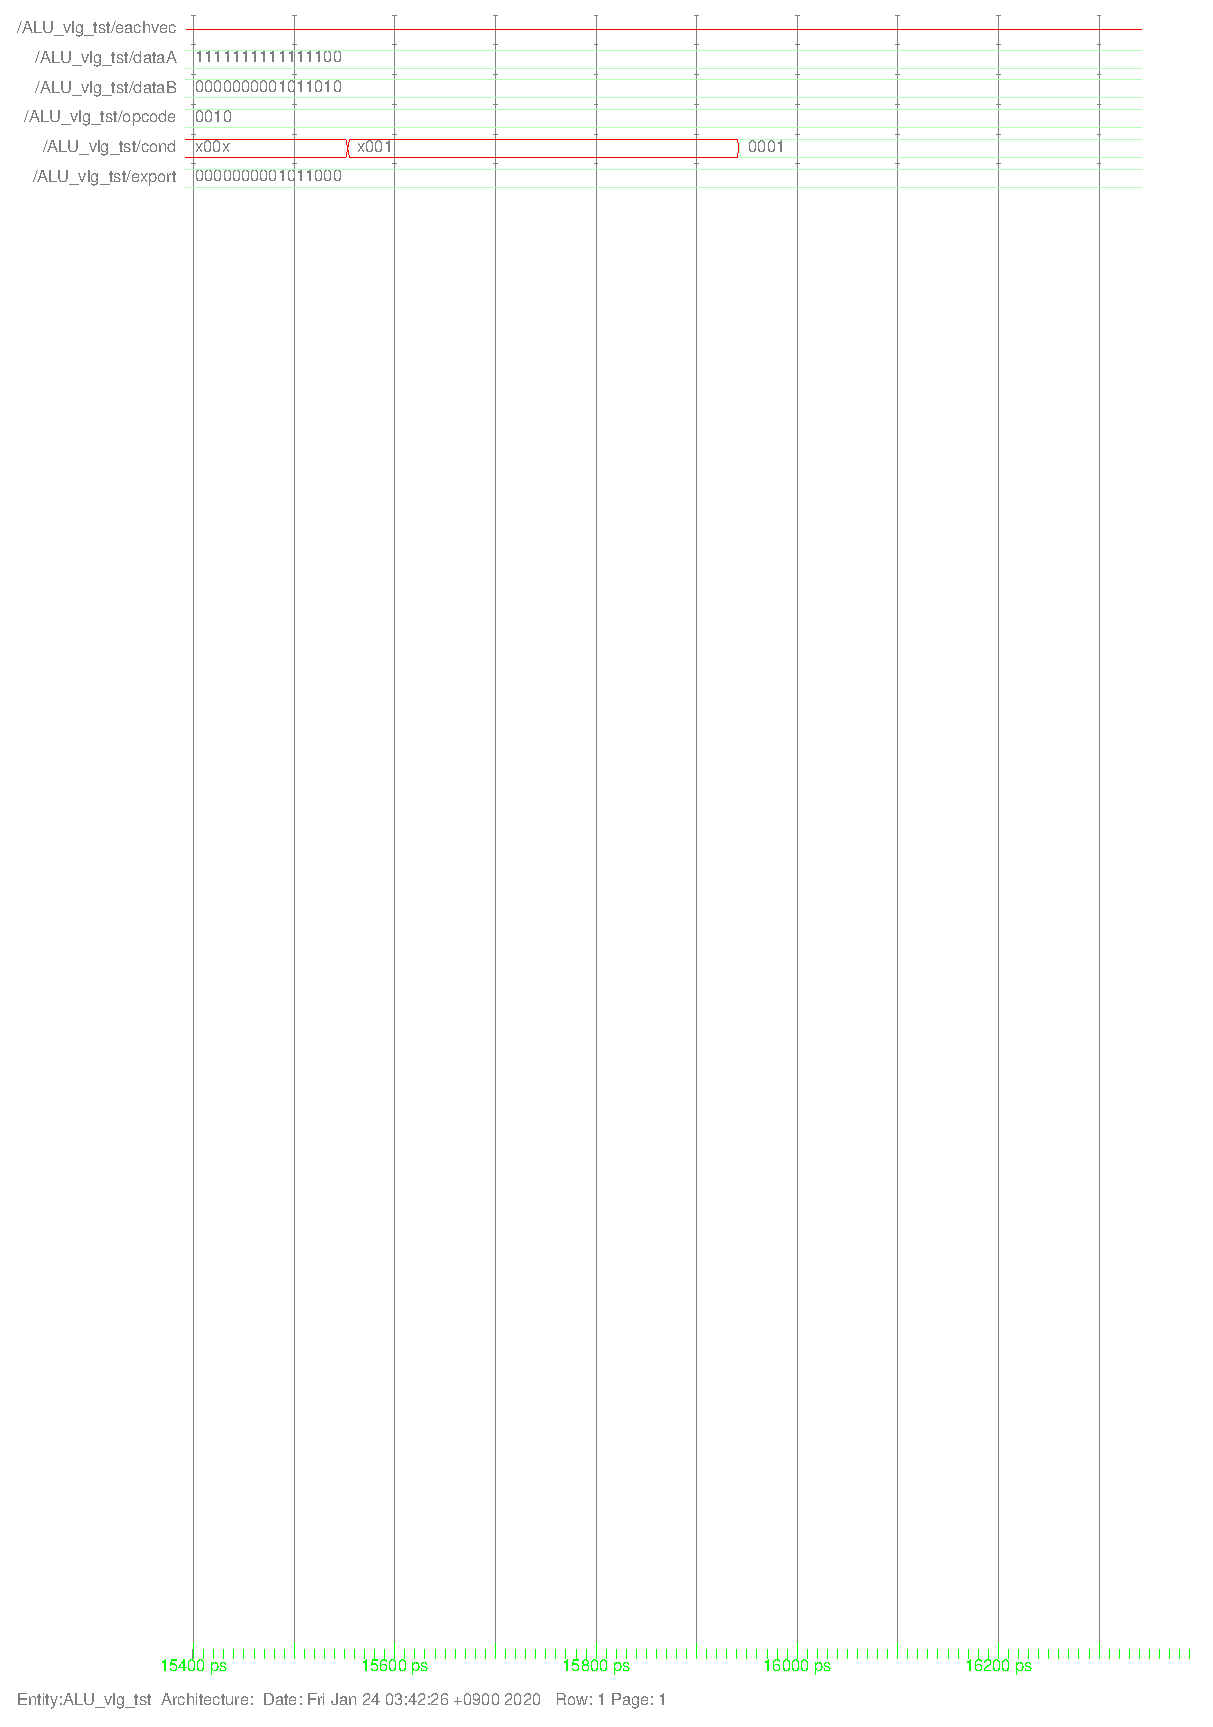
\includegraphics[scale=0.8]{ALU_and.ps}
\end{figure}
\subsection{論理和}
特に言及することはなく図から正しい結果が返されていることがわかる。
\begin{figure}
    \caption{論理和}
  \includegraphics[scale=0.8]{ALU_or.ps}
\end{figure}
\subsection{排他的論理和}
図から各ビットについてちゃんと排他的論理和がとられていることがわかる。
\begin{figure}
    \caption{排他的論理和}
  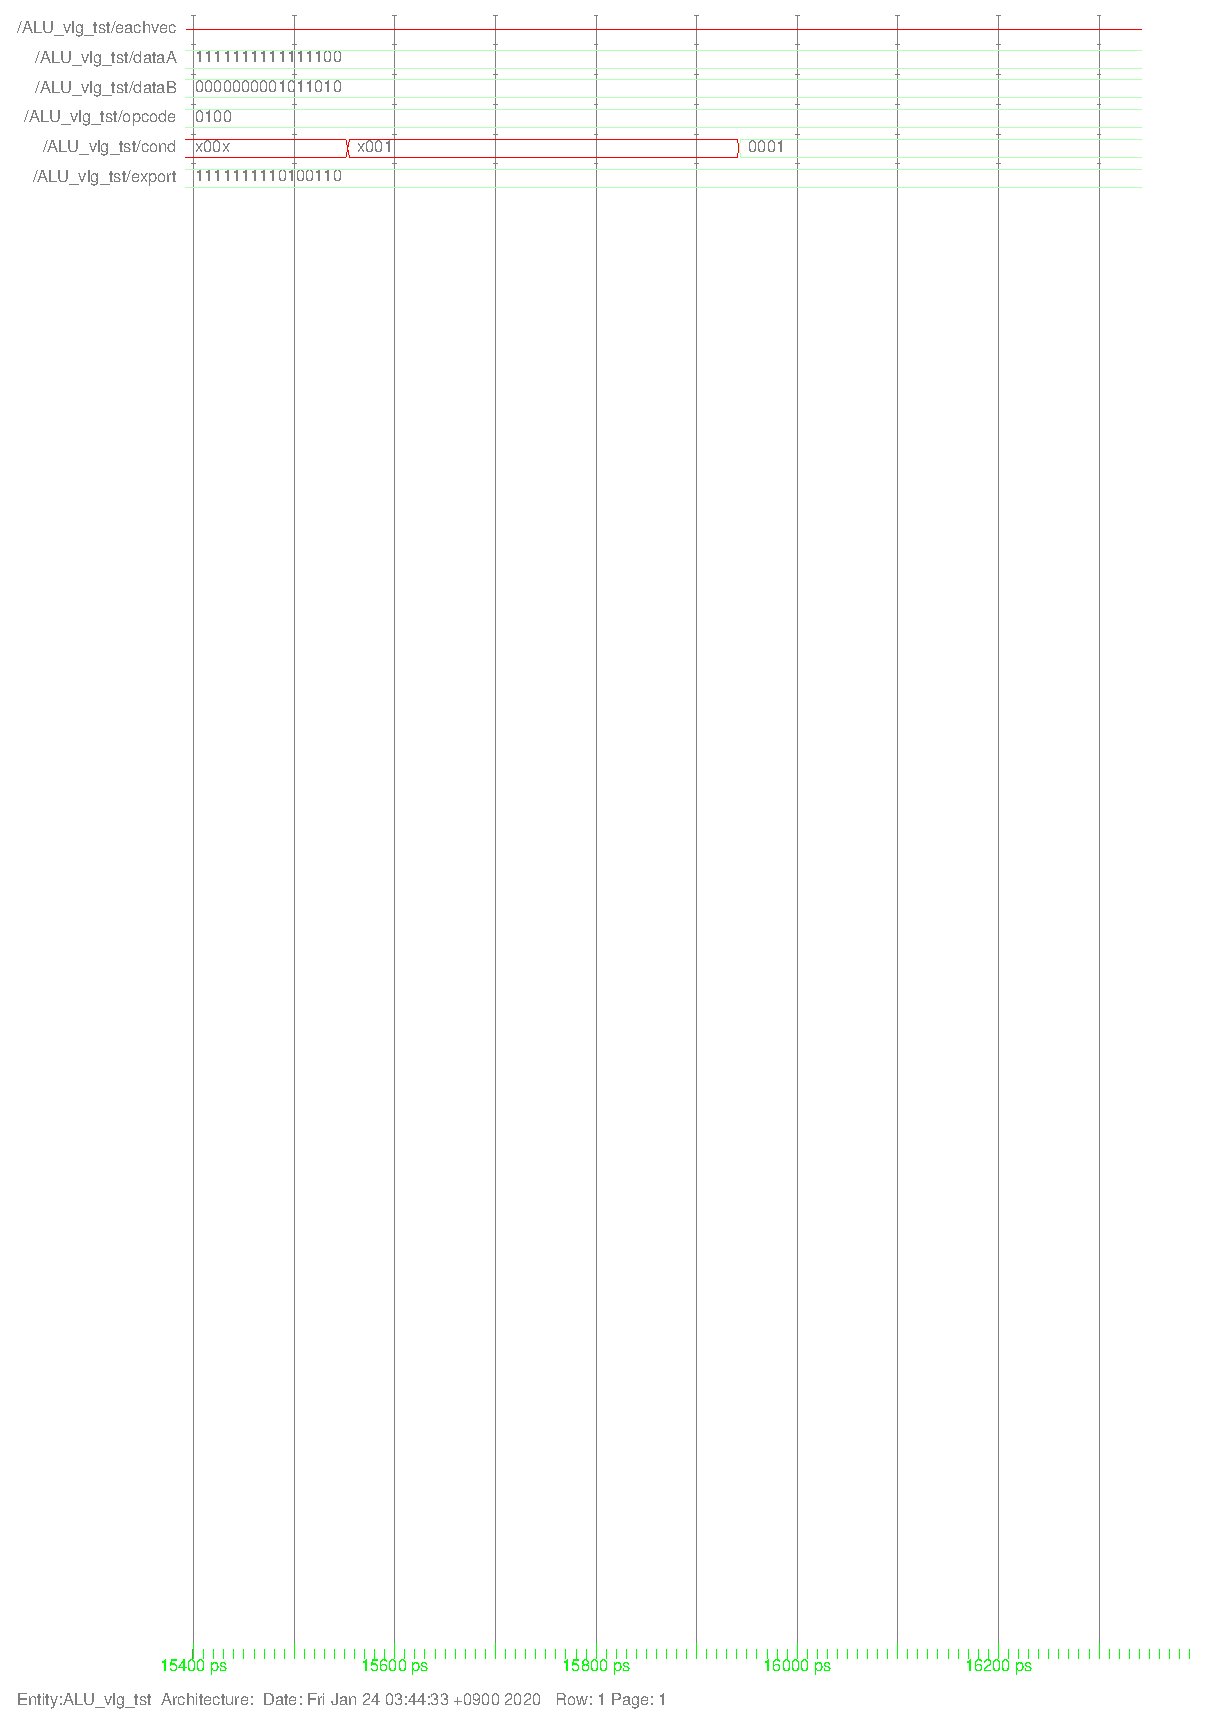
\includegraphics[scale=0.8]{ALU_xor.ps}
\end{figure}
\subsection{比較演算}
等しい入力を与えるとZに1がたっていることがわかる。
\begin{figure}
    \caption{比較演算}
  \includegraphics[scale=0.8]{ALU_cmp.ps}
\end{figure}
\subsection{移動演算}
dataAの中身がそのまま出力されていることがわかる。
\begin{figure}
    \caption{移動演算}
  \includegraphics[scale=0.8]{ALU_mv.ps}
\end{figure}
\subsection{オーバーフロー}
加算についてオーバーフローする例についてシミュレーションした結果、condのオーバーフローフラグにちゃんと1がたっていることが確認できる。
\begin{figure}
    \caption{オーバーフロー}
  \includegraphics[scale=0.8]{ALU_ovf.ps}
\end{figure}

\subsection{改良案(先見回路を用いた例)}
上記のALUでは桁上げ伝搬加算器を用いてALUを構成したため、論理素子が多段接続される数が多くなり遅延が大きくなる。これを解消するためには桁上げ先見加算器を用いた構成を用いることが考えられる。これは桁上げ信号が伝播する論理段数を減らすことで高速化を図るものである。
回路規模を気にしなければ当然16ビット先見加算器を用いればよいのだが、桁数が大きくなるとキャリーを事前に求めるための論理回路が大きくなるので現実的には4ビット先見加算器程度にするのが良いだろう。
回路規模の点では桁上げ伝播加算器の方が性能が良いといえるが、計算時間に関しては桁上げ先見加算器のほうが性能が良いといえる。
\url{https://ocw.kyoto-u.ac.jp/ja/09-faculty-of-engineering-jp/computer-architecture-basics/pdf/slide6.pdf}
によると、桁数をnとして、桁上げ伝搬加算器においてはオーダーはO(n),桁上げ先見加算器についてはO(log n)である。

\section{ALUを用いた同期式順序回路の設計(1001の検出)}
この課題では上で作ったALUを用いて順序回路を作成した。
使った機能は必須機能に限って簡単な単語を受理する順序機械を構成した。クロックに合わせて入力を入れてやらないと入力が何回も読み込まれるようになっているため、テストベンチファイルのほうで上手く調整することで対応した。
\subsection{期待される機能}
入力列$x_{0}x_{1}...x_{n}$に対して、$x_{i}x_{i+1}x_{i+2}x_{i+3} = 1001$という入力が含まれる場合、最後の1を受け取った時に1を出力する。
今回受理する語を1001としたのに特に理由はないが、このような順序機械と同様に様々な入力を検出する順序機械が作れ、0,1の組み合わせからなる語に適当に言語を割り当てておけば、ある言葉が発せられた時に1を出力するような順序機械が作れる。
また、この順序機械では入力の順番が大事なので1,0の組み合わせからなるパスワードを受理する機械として応用することもできる。
\subsection{シミュレーションによって確認できた機能}
\begin{figure}
    \caption{順序機械のシミュレーション}
  \includegraphics[scale=0.8]{pattern_match_1001.ps}
\end{figure}

\begin{table}
    \caption{順序回路の入力と遷移,出力}
    \centering
    \begin{tabular}{|c|c|c||c|c|c|}\hline
        $Q_0$&$Q_1$&$x$&$Q_{0}^{+}$&$Q_{1}^{+}$&$y$ \\ \hline \hline
        0&0&0&0&0&0 \\ \hline
        0&0&1&0&1&0 \\ \hline
        0&1&0&1&0&0 \\ \hline
        0&1&1&0&1&0 \\ \hline
        1&0&0&1&1&0 \\ \hline
        1&0&1&0&1&0 \\ \hline
        1&1&0&0&0&0 \\ \hline
        1&1&1&0&1&1 \\ \hline
    \end{tabular}
\end{table}
上の表は論理式表現にすると、
\begin{equation}
    Q_{0}^{+} = (Q_{0} \oplus Q_{1})x^{'}
\end{equation}
\begin{equation}
    Q_{1}^{+} = Q_{0}Q_{1}^{'} + x
\end{equation}
\begin{equation}
    y = Q_{0}Q_{1}x
\end{equation}
と表せる。
図1に示した波形シミュレーションだけではわかりにくいので、各サイクルでの$x$の値を以下にまとめる。

入力:$1 \rightarrow 0 \rightarrow 0 \rightarrow 1 \rightarrow 0 \rightarrow 0 \rightarrow 1 \rightarrow 0$

これと図の状態遷移及び出力の変化から状態遷移と出力に関して、真理値表及び、論理式に合致した波形であることが読み取れる。
すなわち出力が1となるのは1001が入力されたときであることがわかる。

\subsection{クロック周波数についての考察}
Compilation Reportから読み取れた情報として、Fmaxが1123.6MHzであった。これはクロックがとる値として可能な最大の値を示している。この値が大きい程1サイクルを高速にすることができる。これよりも速い周波数で動作させてしまうと、回路の遅延のために変化が伝わる前に次の素子へと情報が流れてしまい誤動作の原因となる。
\subsection{回路規模の考察}
使った論理素子の数についてCompilation Reportから3 / 28,848 ( $\leq$ 1 \% )という値を得た。これは十分に小さい値であると考えられる。
今回は作った回路が小規模であるので遅延時間もそんなに問題にならなかったと思われるが、回路の大きさがk倍になった時に桁上げ伝播加算器を用いたALUと桁上げ先見加算器を用いたALUでは桁上げ伝播方式ではk倍の計算量がかかるが、桁上げ先見方式では$1 + \frac{\log{k}}{\log{n}}$倍で抑えられるので今回のように回路規模が大きくならないような回路の場合、桁上げ先遣方式を使ったほうが良いと思われる。

\section{参考文献}
Computer Organization and Design MIPS Edition, Fifth Edition: The Hardware/Software Interface (The Morgan Kaufmann Series in Computer Architecture and Design)

https://ocw.kyoto-u.ac.jp/ja/09-faculty-of-engineering-jp/computer-architecture-basics/pdf/slide6.pdf
\end{document}